\documentclass[12pt]{article}

\usepackage{float}
\usepackage{graphicx}			% Use this package to include images
\usepackage{amsmath}			% A library of many standard math expressions
\usepackage[margin=1in]{geometry}% Sets 1in margins. 
\usepackage{fancyhdr}			% Creates headers and footers
\usepackage{enumerate}          %These two package give custom labels to a list
\usepackage[shortlabels]{enumitem}
\usepackage{matlab-prettifier}
\usepackage{tikz}
\usepackage[utf8]{inputenc}
\usepackage{pgfplots} 
\usepackage{pgfgantt}
\usepackage{pdflscape}
\usepackage{array,multirow}
\usepackage{tabularx,booktabs}
\newcolumntype{Y}{>{\centering\arraybackslash}X}
\usetikzlibrary{shapes.geometric}
\usetikzlibrary{arrows.meta,arrows}
\pgfplotsset{compat=newest} 
\pgfplotsset{plot coordinates/math parser=false}
\newlength\fwidth
\newlength\fheight
\usepackage{float,graphicx}
\pagestyle{fancy}
\fancyhead[l]{}
\fancyhead[c]{Experiment 6}
\fancyhead[r]{}
\fancyfoot[c]{\thepage}
\setlength{\headheight}{20pt}
\begin{document}
\author{}
\date{}
\title{Michelson's Interferometer}
\maketitle
\section*{Aim}
To measure the wavelength of a laser, refractive index of glass slide  and air.
\section*{Analysis}
A beam of light passes through a beam splitter (glass slab at $45^\circ$) and reflects off from two mirors.
If all the equipment was arranged ideally, then the ray diagram of the setup would look like the diagram shown below.
Thus, point sources of light would appear to be two dots on the screen.
On inserting a divergence lens in front of the source, we convert the point source into a plane wavefront.
Thus, when the light sources reach the screen, the phases are different and are centered around the two dots.
The resulting shapes that are formed due to these points have the property that the difference between all these points with each of the two dots mentioned before is a constant.
\begin{figure}[H]
    \centering
    \begin{tikzpicture}
        \fill[yellow](-2,-2) -- (2,2) -- (1,3) -- (-3,-1) -- cycle;
        \draw[dashed] (-1,1) -- (1,1) -- (1,-3);
        \draw[dashed] (1,1) -- (3,1);
        \draw[dashed] (1,3) -- (1,1);
        \draw[dashed] (0.5,1) -- (0.5,-3);
        \draw[dashed] (-1,3) -- (-1,-3);
        \draw[thick][->] (-1,3) -- (-1,1) -- (-0.5,-0.5) -- (-0.5,-3);
        \draw[dashed] (-1,0) -- (0,0) -- (0,1);
        \draw[dashed] (0,0) -- (-1,1);
        \draw[thick][->] (-4,1) --(-2.5,1);
        \draw[thick] (-2.5,1) -- (-1,1);
        \draw[thick] (-1,1) -- (0.5,0.5) -- (3,0.5);
        \draw[thick][->] (0.5,0.5) -- (0.5,-3);
        
        \draw[|-|] (0.5,-3.15) -- 
        node[fill=white,inner sep=0.5mm,outer sep=0.5mm] {\small $d$} (1,-3.15);
        \draw[|-|] (3.15,0.5) -- 
        node[fill=white,inner sep=0.5mm,outer sep=0.5mm] {\small $d$} (3.15,1);
        \draw[|-|] (-1,-3.15) -- 
        node[fill=white,inner sep=0.5mm,outer sep=0.5mm] {\small $d$} (-0.5,-3.15);
        \draw[|-|] (1,3.15) -- 
        node[fill=white,inner sep=0.5mm,outer sep=0.5mm] {\small $t\sqrt{2}$} (-1,3.15);
        \draw[|-|] (-2.15,-2.15) -- 
        node[fill=white,inner sep=0.5mm,outer sep=0.5mm] {\small $t$} (-3.15,-1.15);
        \node[circle,inner sep=1pt,fill=red,label=left:{Source}] at (-4,1) {};
    \end{tikzpicture}
    \caption{Here's some text}
\end{figure} 
This is the definition of a hyperbola.
Thus, the screen makes hyperbolic fringes with the foci as the two dots.
The distance between the dots is the two times the focal length of the hyperbolic fringes (which is $t\sqrt{2}-2d$).
When we adjust the settings so that both these points converge to the same point, the focal length becomes zero which results in the equation of a circle. This is how we get circular fringes and any deviation results in hyperbolic fringes.
\pagebreak

The wavelength of the laser is calculated by \(\lambda = (2d/N)\Delta\) where $\Delta$ is the caliberation constant of the micrometer and $d$ is the micrometer reading.
We first find $\Delta$ by using green laser of wavelength $532 \text{ }nm$.
We find it to be $0.02325$
\subsection*{Calculating values}
\begin{enumerate}
    \item For wavelength of red light
    \[\lambda_r = \lambda_g\times \frac{d_r}{d_g}\]
    This gives us the value for wavelength of red laser as $643.6\text{ }nm$
    \item For refractive index of glass slide
    \[n =\frac{(2t-N\lambda)(1-\cos \theta)}{2t(1-\cos \theta)-N\lambda}\]
    Which gives us refractive index as 1.592
    \item For refractive index of air
    \begin{figure}[H]
        \centering
        \setlength\fwidth{0.75\textwidth}
        \setlength\fheight{0.5\textwidth}
        % This file was created by matlab2tikz.
%
\definecolor{mycolor1}{rgb}{0.00000,0.44700,0.74100}%
\definecolor{mycolor2}{rgb}{0.85000,0.32500,0.09800}%
\definecolor{mycolor3}{rgb}{0.12941,0.12941,0.12941}%
%
\begin{tikzpicture}

\begin{axis}[%
width=0.951\fwidth,
height=\fheight,
at={(0\fwidth,0\fheight)},
scale only axis,
xmin=0,
xmax=300,
xlabel style={font=\color{mycolor3}},
xlabel={Pressure (in mmHg)},
ymin=0,
ymax=30,
ylabel style={font=\color{mycolor3}},
ylabel={Number of fringes},
axis background/.style={fill=white},
xmajorgrids,
ymajorgrids,
legend style={legend cell align=left, align=left}
]
\addplot[only marks, mark=o, mark options={}, mark size=1.5000pt, draw=mycolor1] table[row sep=crcr]{%
x	y\\
300	0\\
260	3\\
225	6\\
190	9\\
155	12\\
120	15\\
85	18\\
50	21\\
15	24\\
};
\addlegendentry{Data}

\addplot [color=mycolor2]
  table[row sep=crcr]{%
0	25.2048\\
1.00286532951289	25.1196687679083\\
2.00573065902579	25.0345375358166\\
3.00859598853868	24.9494063037249\\
4.01146131805158	24.8642750716332\\
5.01432664756447	24.7791438395415\\
6.01719197707736	24.6940126074499\\
7.02005730659026	24.6088813753582\\
8.02292263610315	24.5237501432665\\
9.02578796561605	24.4386189111748\\
10.0286532951289	24.3534876790831\\
11.0315186246418	24.2683564469914\\
12.0343839541547	24.1832252148997\\
13.0372492836676	24.098093982808\\
14.0401146131805	24.0129627507163\\
15.0429799426934	23.9278315186246\\
16.0458452722063	23.8427002865329\\
17.0487106017192	23.7575690544413\\
18.0515759312321	23.6724378223496\\
19.054441260745	23.5873065902579\\
20.0573065902579	23.5021753581662\\
21.0601719197708	23.4170441260745\\
22.0630372492837	23.3319128939828\\
23.0659025787966	23.2467816618911\\
24.0687679083095	23.1616504297994\\
25.0716332378224	23.0765191977077\\
26.0744985673352	22.991387965616\\
27.0773638968481	22.9062567335244\\
28.080229226361	22.8211255014327\\
29.0830945558739	22.735994269341\\
30.0859598853868	22.6508630372493\\
31.0888252148997	22.5657318051576\\
32.0916905444126	22.4806005730659\\
33.0945558739255	22.3954693409742\\
34.0974212034384	22.3103381088825\\
35.1002865329513	22.2252068767908\\
36.1031518624642	22.1400756446991\\
37.1060171919771	22.0549444126074\\
38.10888252149	21.9698131805158\\
39.1117478510029	21.8846819484241\\
40.1146131805158	21.7995507163324\\
41.1174785100287	21.7144194842407\\
42.1203438395415	21.629288252149\\
43.1232091690544	21.5441570200573\\
44.1260744985673	21.4590257879656\\
45.1289398280802	21.3738945558739\\
46.1318051575931	21.2887633237822\\
47.134670487106	21.2036320916905\\
48.1375358166189	21.1185008595989\\
49.1404011461318	21.0333696275072\\
50.1432664756447	20.9482383954155\\
51.1461318051576	20.8631071633238\\
52.1489971346705	20.7779759312321\\
53.1518624641834	20.6928446991404\\
54.1547277936963	20.6077134670487\\
55.1575931232092	20.522582234957\\
56.1604584527221	20.4374510028653\\
57.163323782235	20.3523197707736\\
58.1661891117478	20.2671885386819\\
59.1690544412607	20.1820573065903\\
60.1719197707736	20.0969260744986\\
61.1747851002865	20.0117948424069\\
62.1776504297994	19.9266636103152\\
63.1805157593123	19.8415323782235\\
64.1833810888252	19.7564011461318\\
65.1862464183381	19.6712699140401\\
66.189111747851	19.5861386819484\\
67.1919770773639	19.5010074498567\\
68.1948424068768	19.415876217765\\
69.1977077363897	19.3307449856733\\
70.2005730659026	19.2456137535817\\
71.2034383954155	19.16048252149\\
72.2063037249284	19.0753512893983\\
73.2091690544413	18.9902200573066\\
74.2120343839541	18.9050888252149\\
75.214899713467	18.8199575931232\\
76.2177650429799	18.7348263610315\\
77.2206303724928	18.6496951289398\\
78.2234957020057	18.5645638968481\\
79.2263610315186	18.4794326647564\\
80.2292263610315	18.3943014326648\\
81.2320916905444	18.3091702005731\\
82.2349570200573	18.2240389684814\\
83.2378223495702	18.1389077363897\\
84.2406876790831	18.053776504298\\
85.243553008596	17.9686452722063\\
86.2464183381089	17.8835140401146\\
87.2492836676218	17.7983828080229\\
88.2521489971347	17.7132515759312\\
89.2550143266476	17.6281203438395\\
90.2578796561605	17.5429891117479\\
91.2607449856734	17.4578578796562\\
92.2636103151862	17.3727266475645\\
93.2664756446991	17.2875954154728\\
94.269340974212	17.2024641833811\\
95.2722063037249	17.1173329512894\\
96.2750716332378	17.0322017191977\\
97.2779369627507	16.947070487106\\
98.2808022922636	16.8619392550143\\
99.2836676217765	16.7768080229226\\
100.286532951289	16.6916767908309\\
101.289398280802	16.6065455587393\\
102.292263610315	16.5214143266476\\
103.295128939828	16.4362830945559\\
104.297994269341	16.3511518624642\\
105.300859598854	16.2660206303725\\
106.303724928367	16.1808893982808\\
107.30659025788	16.0957581661891\\
108.309455587393	16.0106269340974\\
109.312320916905	15.9254957020057\\
110.315186246418	15.840364469914\\
111.318051575931	15.7552332378223\\
112.320916905444	15.6701020057307\\
113.323782234957	15.584970773639\\
114.32664756447	15.4998395415473\\
115.329512893983	15.4147083094556\\
116.332378223496	15.3295770773639\\
117.335243553009	15.2444458452722\\
118.338108882521	15.1593146131805\\
119.340974212034	15.0741833810888\\
120.343839541547	14.9890521489971\\
121.34670487106	14.9039209169054\\
122.349570200573	14.8187896848138\\
123.352435530086	14.7336584527221\\
124.355300859599	14.6485272206304\\
125.358166189112	14.5633959885387\\
126.361031518625	14.478264756447\\
127.363896848138	14.3931335243553\\
128.36676217765	14.3080022922636\\
129.369627507163	14.2228710601719\\
130.372492836676	14.1377398280802\\
131.375358166189	14.0526085959885\\
132.378223495702	13.9674773638968\\
133.381088825215	13.8823461318052\\
134.383954154728	13.7972148997135\\
135.386819484241	13.7120836676218\\
136.389684813754	13.6269524355301\\
137.392550143266	13.5418212034384\\
138.395415472779	13.4566899713467\\
139.398280802292	13.371558739255\\
140.401146131805	13.2864275071633\\
141.404011461318	13.2012962750716\\
142.406876790831	13.1161650429799\\
143.409742120344	13.0310338108882\\
144.412607449857	12.9459025787966\\
145.41547277937	12.8607713467049\\
146.418338108883	12.7756401146132\\
147.421203438395	12.6905088825215\\
148.424068767908	12.6053776504298\\
149.426934097421	12.5202464183381\\
150.429799426934	12.4351151862464\\
151.432664756447	12.3499839541547\\
152.43553008596	12.264852722063\\
153.438395415473	12.1797214899713\\
154.441260744986	12.0945902578797\\
155.444126074499	12.009459025788\\
156.446991404011	11.9243277936963\\
157.449856733524	11.8391965616046\\
158.452722063037	11.7540653295129\\
159.45558739255	11.6689340974212\\
160.458452722063	11.5838028653295\\
161.461318051576	11.4986716332378\\
162.464183381089	11.4135404011461\\
163.467048710602	11.3284091690544\\
164.469914040115	11.2432779369627\\
165.472779369628	11.1581467048711\\
166.47564469914	11.0730154727794\\
167.478510028653	10.9878842406877\\
168.481375358166	10.902753008596\\
169.484240687679	10.8176217765043\\
170.487106017192	10.7324905444126\\
171.489971346705	10.6473593123209\\
172.492836676218	10.5622280802292\\
173.495702005731	10.4770968481375\\
174.498567335244	10.3919656160458\\
175.501432664756	10.3068343839542\\
176.504297994269	10.2217031518625\\
177.507163323782	10.1365719197708\\
178.510028653295	10.0514406876791\\
179.512893982808	9.96630945558739\\
180.515759312321	9.8811782234957\\
181.518624641834	9.79604699140401\\
182.521489971347	9.71091575931232\\
183.52435530086	9.62578452722063\\
184.527220630372	9.54065329512894\\
185.530085959885	9.45552206303725\\
186.532951289398	9.37039083094556\\
187.535816618911	9.28525959885387\\
188.538681948424	9.20012836676218\\
189.541547277937	9.11499713467049\\
190.54441260745	9.02986590257879\\
191.547277936963	8.9447346704871\\
192.550143266476	8.85960343839541\\
193.553008595989	8.77447220630372\\
194.555873925501	8.68934097421203\\
195.558739255014	8.60420974212034\\
196.561604584527	8.51907851002865\\
197.56446991404	8.43394727793696\\
198.567335243553	8.34881604584527\\
199.570200573066	8.26368481375358\\
200.573065902579	8.17855358166189\\
201.575931232092	8.0934223495702\\
202.578796561605	8.00829111747851\\
203.581661891117	7.92315988538682\\
204.58452722063	7.83802865329513\\
205.587392550143	7.75289742120344\\
206.590257879656	7.66776618911175\\
207.593123209169	7.58263495702005\\
208.595988538682	7.49750372492836\\
209.598853868195	7.41237249283667\\
210.601719197708	7.32724126074498\\
211.604584527221	7.24211002865329\\
212.607449856734	7.1569787965616\\
213.610315186246	7.07184756446991\\
214.613180515759	6.98671633237822\\
215.616045845272	6.90158510028653\\
216.618911174785	6.81645386819484\\
217.621776504298	6.73132263610315\\
218.624641833811	6.64619140401146\\
219.627507163324	6.56106017191977\\
220.630372492837	6.47592893982808\\
221.63323782235	6.39079770773639\\
222.636103151862	6.3056664756447\\
223.638968481375	6.22053524355301\\
224.641833810888	6.13540401146131\\
225.644699140401	6.05027277936962\\
226.647564469914	5.96514154727793\\
227.650429799427	5.88001031518624\\
228.65329512894	5.79487908309455\\
229.656160458453	5.70974785100286\\
230.659025787966	5.62461661891117\\
231.661891117479	5.53948538681948\\
232.664756446991	5.45435415472779\\
233.667621776504	5.3692229226361\\
234.670487106017	5.28409169054441\\
235.67335243553	5.19896045845272\\
236.676217765043	5.11382922636103\\
237.679083094556	5.02869799426934\\
238.681948424069	4.94356676217765\\
239.684813753582	4.85843553008596\\
240.687679083095	4.77330429799427\\
241.690544412607	4.68817306590258\\
242.69340974212	4.60304183381089\\
243.696275071633	4.51791060171919\\
244.699140401146	4.4327793696275\\
245.702005730659	4.34764813753581\\
246.704871060172	4.26251690544412\\
247.707736389685	4.17738567335243\\
248.710601719198	4.09225444126074\\
249.713467048711	4.00712320916905\\
250.716332378223	3.92199197707736\\
251.719197707736	3.83686074498567\\
252.722063037249	3.75172951289398\\
253.724928366762	3.66659828080229\\
254.727793696275	3.5814670487106\\
255.730659025788	3.49633581661891\\
256.733524355301	3.41120458452722\\
257.736389684814	3.32607335243553\\
258.739255014327	3.24094212034383\\
259.74212034384	3.15581088825215\\
260.744985673352	3.07067965616045\\
261.747851002865	2.98554842406876\\
262.750716332378	2.90041719197708\\
263.753581661891	2.81528595988538\\
264.756446991404	2.73015472779369\\
265.759312320917	2.645023495702\\
266.76217765043	2.55989226361031\\
267.765042979943	2.47476103151863\\
268.767908309456	2.38962979942693\\
269.770773638968	2.30449856733524\\
270.773638968481	2.21936733524355\\
271.776504297994	2.13423610315186\\
272.779369627507	2.04910487106017\\
273.78223495702	1.96397363896848\\
274.785100286533	1.87884240687679\\
275.787965616046	1.7937111747851\\
276.790830945559	1.7085799426934\\
277.793696275072	1.62344871060172\\
278.796561604585	1.53831747851002\\
279.799426934097	1.45318624641833\\
280.80229226361	1.36805501432665\\
281.805157593123	1.28292378223495\\
282.808022922636	1.19779255014327\\
283.810888252149	1.11266131805158\\
284.813753581662	1.02753008595988\\
285.816618911175	0.942398853868195\\
286.819484240688	0.857267621776501\\
287.822349570201	0.77213638968481\\
288.825214899713	0.687005157593124\\
289.828080229226	0.60187392550143\\
290.830945558739	0.516742693409739\\
291.833810888252	0.431611461318045\\
292.836676217765	0.346480229226358\\
293.839541547278	0.261348997134668\\
294.842406876791	0.176217765042974\\
295.845272206304	0.0910865329512873\\
296.848137535817	0.00595530085959695\\
297.85100286533	-0.0791759312320934\\
298.853868194842	-0.164307163323784\\
299.856733524355	-0.249438395415478\\
300.859598853868	-0.334569627507165\\
301.862464183381	-0.419700859598855\\
302.865329512894	-0.504832091690549\\
303.868194842407	-0.589963323782236\\
304.87106017192	-0.67509455587393\\
305.873925501433	-0.76022578796562\\
306.876790830946	-0.845357020057307\\
307.879656160458	-0.930488252149001\\
308.882521489971	-1.01561948424069\\
309.885386819484	-1.10075071633239\\
310.888252148997	-1.18588194842407\\
311.89111747851	-1.27101318051576\\
312.893982808023	-1.35614441260745\\
313.896848137536	-1.44127564469914\\
314.899713467049	-1.52640687679083\\
315.902578796562	-1.61153810888252\\
316.905444126074	-1.69666934097421\\
317.908309455587	-1.78180057306591\\
318.9111747851	-1.86693180515759\\
319.914040114613	-1.95206303724929\\
320.916905444126	-2.03719426934098\\
321.919770773639	-2.12232550143267\\
322.922636103152	-2.20745673352436\\
323.925501432665	-2.29258796561605\\
324.928366762178	-2.37771919770774\\
325.931232091691	-2.46285042979943\\
326.934097421203	-2.54798166189112\\
327.936962750716	-2.63311289398281\\
328.939828080229	-2.7182441260745\\
329.942693409742	-2.80337535816619\\
330.945558739255	-2.88850659025788\\
331.948424068768	-2.97363782234957\\
332.951289398281	-3.05876905444126\\
333.954154727794	-3.14390028653295\\
334.957020057307	-3.22903151862464\\
335.95988538682	-3.31416275071634\\
336.962750716332	-3.39929398280803\\
337.965616045845	-3.48442521489972\\
338.968481375358	-3.56955644699141\\
339.971346704871	-3.6546876790831\\
340.974212034384	-3.73981891117479\\
341.977077363897	-3.82495014326648\\
342.97994269341	-3.91008137535817\\
343.982808022923	-3.99521260744986\\
344.985673352436	-4.08034383954155\\
345.988538681948	-4.16547507163324\\
346.991404011461	-4.25060630372493\\
347.994269340974	-4.33573753581662\\
348.997134670487	-4.42086876790831\\
350	-4.506\\
};
\addlegendentry{Fit}

\end{axis}
\end{tikzpicture}%
    \end{figure}
    \[n = 1 + \frac{m}{\Delta P}\cdot \frac{\lambda}{2l}\cdot P_{atm}\] where $l$ is the length of the pressure cell (8.02 cm) and $m$ is the number change in fringes.
    We get the value as 1.00024
\end{enumerate}
\subsection*{Calculating errors}
If $f$ is a function of $x_i$s then the uncertainty in $f$ is given by
\[\sigma_f^2=\sum_{i = 1}^{n} \bigg(\frac{\partial f}{\partial x_i}\sigma_{x_i}\bigg)^2 \]
Let $p = 1-\cos\theta$

\noindent The uncertainties are
\begin{align*}
    \sigma_{d_r/d_g} &= 0.034\\
    \sigma_p &= \sin\theta\cdot\sigma_\theta = 0.19
\end{align*}
\begin{align*}
\end{align*}
\begin{enumerate}
    \item For wavelength of red light
    \[\sigma_\lambda = \lambda_g\cdot\sigma_{d_r/d_g} = 18.4\]
    \item For refractive index of glass slide
    \[\sigma_n=\sqrt{\bigg(\frac{(N\lambda -2t)(N\lambda)}{(2tp-N\lambda)^2}\cdot\sigma_p \bigg)^2 + \bigg(\frac{2tpN(1-p)}{(2tp-N\lambda)^2}\cdot\sigma_\lambda\bigg)^2} = 0.22\]
    \item For refractive index of air
    \[\sigma_n =\frac{m}{\Delta P}\cdot \frac{P_{atm}}{2l}\cdot\sigma_\lambda = 7.2\times 10^{-6}\]
\end{enumerate}
\section*{Result}
We obtain the following results
\begin{enumerate}
    \item The wavelength of red light is $643.6\pm 18.4$ nm
    \item The refractive index of glass slide is $1.592\pm 0.22$
    \item The refractive index of air is 1.00024
\end{enumerate}
\end{document}  